\documentclass{article}

\usepackage[hidelinks]{hyperref}

\usepackage{tikz}
\usetikzlibrary{matrix,chains,positioning,decorations.pathreplacing,arrows}

\usepackage[color=cyan]{todonotes}

\usepackage{minted}
\usemintedstyle{colorful}

\usepackage{graphicx}
\graphicspath{{./images/}}

\usepackage[T1]{fontenc}
\usepackage{verbatim}

\addtolength{\oddsidemargin}{-.875in}
\addtolength{\evensidemargin}{-.875in}
\addtolength{\textwidth}{1.75in}

\addtolength{\topmargin}{-.875in}
\addtolength{\textheight}{1.75in}

\bibliographystyle{plain}

\begin{document}

\title{To What Extent Can a Neural Network Be Used to Differentiate Between Programming Languages Through Textual Analysis?}
\author{Erik Boesen, Candidate gsg256}

\maketitle

\begin{abstract}
The notion of ``Artificial Intelligence'' evokes in the public mind a variety of reactions, from excitement at the prospect of driverless cars to guttural fear of a robot uprising. Despite these lofty goals and ethical concerns, applications of AI are and have long been present throughout society. Smartphone owners have their physical locations, web traffic, and social interactions monitored by advertisers. When taking a plane flight, passengers rest safely in the hands of an artificially intelligent autopilot, enjoying the benefit of a trip automatically scheduled to ensure full seats. Even human drivers are assisted by a mobile map applications which use AI to assess traffic conditions in order to choose an optimal route. One heavily researched branch of AI is known as ``machine learning,'' in which models are trained from sample data to find patterns and learn to perform a task without direct human input. One popular technique of machine learning, the ``neural network,'' is distinguished in that it attempts to simulate the decision-making style of a biological brain in order to adapt and learn much like a human. The field of natural language processing relies heavily on neural networks. However, little research has been done on how neural networks may aid in \textit{artificial} language processing, i.e. programming languages. Here, we explore the extent to which neural networks can be applied to differentiating between 10 different programming languages. We outline the fundamentals of neural network technology, and implement a network which correctly determines the language of code in 84\% of trials.
\end{abstract}

\tableofcontents
\pagebreak

\section{Introduction}
In this research we examine the popular machine learning technique of neural networking, specifically within the area of ``deep'' neural networking. In order to illustrate this technology, we outline and implement a neural network which learns to differentiate between the world's 10 most commonly used programming languages.\footnote{According to the TIOBE Index \cite{tiobe}, a popular index tracking the prevalence of programming languages as measured by search engine queries. The top 10 languages according to the May 2018 iteration of the Index are Java, C, C++, Python, C\#, Visual Basic .NET, PHP, JavaScript, SQL, and Ruby. However, our repository of training data, RosettaCode, has a limited amount of SQL code available. In order to balance the training process out, we have exchanged SQL for R, which comes in at \#11 on the TIOBE index but has more sample source code available.} The learning techniques used are generalizable to any selection of languages, as the neural network we design can be trained with any inputs and are never explicitly instructed of specific syntactic features of any language. In order to perform identification, the network will be fed data on individual blocks of code, and will gradually adjust its weights and biases in order to ``learn'' the attributes of each language without being explicitly instructed. Having learned to distinguish between languages, it will be able to perform this task without further feedback, exhibiting well the manner in which computers are able to be trained through Machine Learning techniques.

\section{Outline of Neural Network technique}
\subsection{Definition and use cases}
For many problems within computer science, a programmer attempts to find the function $f(x)$ mapping one or more variables to an output. For some problems, programmers are able to write trivial code performing human-readable mathematical operations. However, consider problems as complex as recognizing the human language being spoken in an audio file. The difficulty of writing static code to perform this task would be monumental, and this sort of problem is where machine learning shines \cite{10algos}.

Machine learning refers to a broad set of techniques wherein computers, through various mathematical constructs, are able to interpret data, find patterns, and learn to make decisions sans excessive human interference \cite{sasml}. Machine Learning techniques are useful when a large and diverse set of data must be processed (often categorized), but when writing explicit code to make distinctions between data points would be impractical or just plain hard. Another classic example of the utility of Machine Learning techniques is the challenge of image recognition. When identifying objects in an image, as in \cite{hinton12}, an unimaginably large and varied body of image data needs to be taken into account for each input. Without machine learning, a programmer would need to write a prohibitively large amount of esoteric code. If such a task could even be accomplished, the excessive number of edge cases for which this poor developer would need to account would make such an application unimaginably laborious to develop. With the benefit of machine learning, however, a programmer need only instruct his or her computer to look through already-identified images, identifying the qualities of each object class and learning to make distinctions completely on its own.

Though there exist simpler machine learning techniques, such as the classic linear regression or the K Nearest Neighbors algorithm, these strategies have trouble making decisions in so many dimensions of input as demonstrated in \cite{knnic}. For such problems, neural networks are often used and are the subject of much study. Though the notion of a neural network was first proposed in 1958 \cite{rosenblatt58}, this technique has recently experienced a resurgence of popularity. Machine learning techniques based on neural networks including deep learning \cite{mitdeeplearning} and recurrent neural networks \cite{recurrentsurvey} have recently been applied to diverse problems, including achieving victory over a human in the age-old game of Go \cite{go1}\cite{go2}, differentiating between multiple thousands of different image classes \cite{hinton12}, and even recognizing verbal speech \cite{rnnspoken}.

\subsection{Neuron structure}
Simply put, neural networks make complex, nonlinear problems easier by taking cues from neurobiology and simulating how a real brain adapts and makes decisions. In the brains of humans and other animals, many neurons are joined together. These neurons themselves simply take electrical input, adjust it, and pass it along to the next neuron. Biological brains readjust the behavior of their individual constituent neurons, and in doing so are able to learn information and skills.

Though this is an oversimplification of the actual biological processes of learning and neuroplasticity, it may be a helpful metaphor to understand the function of an artificial neural network.

A neural network is composed of several groups (``layers'') of ``neurons.'' Much like in a biological brain, these neurons take input from the previous layer's neurons and use that input to make a decision on what information to itself pass on. The process performed by each neuron during decision making is relatively simple and is thus easier to think about outside the context of a larger network. First, the neuron sums the output values $\xi$ of all neurons from which it receives input, multiplying each input value by a ``weight'' $\omega$. These weights, having been calculated during the process of training the network, essentially represent the importance of the input neuron for making the particular decision on which the network is working. A static or dynamic ``bias'' is added to each neuron which can create a threshold for the neuron to fire. This result then passes through an activation function, which brings the output into a regular range such as $(0, 1)$ or $(-1, 1)$.\footnote{Modern activation functions, such as ReLU, do not place such a limit on their output \cite{activationfunctions}.} There exist many different activation functions, however, in this investigation we use the common $\sigma$ (``sigmoid'') function, which limits our neuron's output to $(0, 1)$:
$$\sigma(x)=\frac{1}{1+e^{-x}}$$
Hence, you may think of the neuron output $\mathcal{O}$ thus:
$$\mathcal{O}=\sigma(\sum_n[w_{n}\xi_{n}]+b)$$
After the activation function is applied, the returned value is given as the neuron's output, and the process is repeated, using that output as the input for successive neurons. A single neuron, hence, might be visualized as follows:\footnote{Original graphic rendering code sourced from \cite{neurondiagrams}.}

\begin{center}
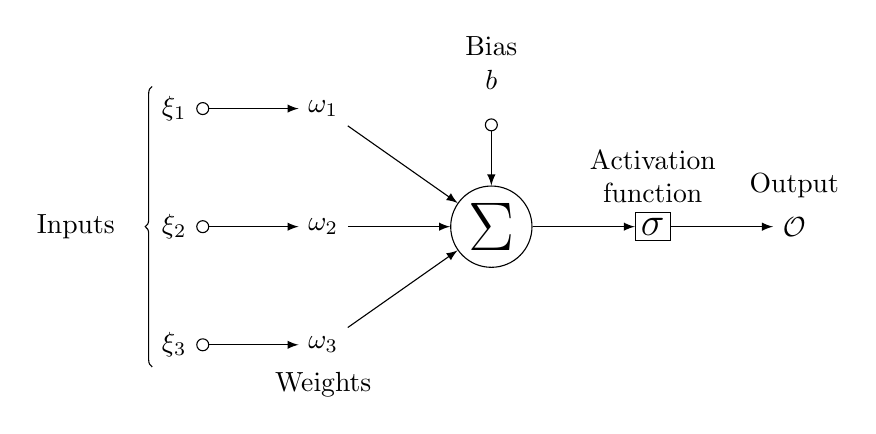
\begin{tikzpicture}[
init/.style={draw, circle, inner sep=2pt, font=\Huge, join = by -latex},
squa/.style={draw, inner sep=2pt, font=\Large, join = by -latex},
start chain=2,node distance=13mm
]
\node[on chain=2] (x2) {$\xi_2$};
\node[on chain=2, join=by o-latex] {$\omega_2$};
\node[on chain=2, init] (sigma) {$\displaystyle\Sigma$};
\node[on chain=2, squa,label=above:{\parbox{2cm}{\centering Activation \\ function}}] {$\sigma$};
\node[on chain=2, label=above:Output,join=by -latex] {$\mathcal{O}$};
\begin{scope}[start chain=1]
  \node[on chain=1] at (0,1.5cm) (x1) {$\xi_1$};
  \node[on chain=1, join=by o-latex] (w1) {$\omega_1$};
\end{scope}
\begin{scope}[start chain=3]
  \node[on chain=3] at (0,-1.5cm) (x3) {$\xi_3$};
  \node[on chain=3, label=below:Weights, join=by o-latex] (w3) {$\omega_3$};
\end{scope}
\node[label=above:\parbox{2cm}{\centering Bias \\ $b$}] at (sigma|-w1) (b) {};

\draw[-latex] (w1) -- (sigma);
\draw[-latex] (w3) -- (sigma);
\draw[o-latex] (b) -- (sigma);

\draw[decorate,decoration={brace,mirror}] (x1.north west) -- node[left=10pt] {Inputs} (x3.south west);
\end{tikzpicture}
\end{center}

\subsection{Network structure}
Understanding now the basic logic behind individual neurons, we turn to the architecture of a full neural network. The most basic network format, known frequently as ``feed forward,'' contains three types of layers, each of which is a vector of neurons, each taking input from every neuron in the previous layer without interacting with the rest of the layer.
\begin{itemize}
\item{The first layer is the \textbf{input layer}. Input data for the network's decision making process, which must be of a consistent size, is fed directly into this layer, and the number of neurons typically is the same as the number of possible input values.}
\item{Following the input layer comes at least one \textbf{hidden layer}. Networks with more than one hidden layer are typically used for more complex problems, and are referred to as ``deep neural networks.'' The output values of the neurons in these layers are not necessarily returned to a user, rather, they are passed on to the following layer, which can be the output layer or another hidden layer.}
\item{Neurons in the \textbf{output layer} return the output of the neural network. Note that traditionally, an activation function is implemented here as well, so basic feed forward networks are generally capable only of outputting a value in the range of the chosen activation function. In some problems, there will be only one output neuron giving a probability, from $0$ to $1$, of some relevant data point $f(x)$ being true. Classification networks designed to distinguish between several categories of input typically use multiple neurons in the output layer giving the probabilities that the input fits into each group.}
\end{itemize}

It may be useful to understand the structure of a neural network through a graphical example \cite{neurondiagrams}, where $\xi_n$ represents a scalar input to the network and $\mathcal{O}$ its single output.
\begin{center}
\begin{tikzpicture}[
plain/.style={draw=none, fill=none},
net/.style={matrix of nodes, nodes={draw, circle, inner sep=8pt}, nodes in empty cells, column sep=2cm, row sep=1pt}, >=latex
]
\matrix[net] (mat)
{
|[plain]| \parbox{1.3cm}{\centering Input\\layer} & |[plain]| \parbox{1.3cm}{\centering Hidden\\layer} & |[plain]| \parbox{1.3cm}{\centering Output\\layer} \\
& |[plain]| \\
|[plain]| & \\
& |[plain]| \\
  |[plain]| & |[plain]| \\
& & \\
  |[plain]| & |[plain]| \\
& |[plain]| \\
  |[plain]| & \\
& |[plain]| \\    };
\foreach \ai [count=\mi ]in {2,4,...,10}
% TODO: Figure out how to actually use TIKZ
% TODO: I just need to turn this in but that doesn't excuse this flagrant abuse of human rights
\node[circle,1.2cm] (mat-\ai-1) at (-4.25,-1.68*\mi+3.9) {$\xi_\mi$} +(0,0);

\foreach \ai in {2,4,...,10}
{\foreach \aii in {3,6,9}
  \draw[->] (mat-\ai-1) -- (mat-\aii-2);
}
\foreach \ai in {3,6,9}
  \draw[->] (mat-\ai-2) -- (mat-6-3);
  \draw[->] (mat-6-3) -- node[above] {$\mathcal{O}$} +(2cm,0);
\end{tikzpicture}
\end{center}

\subsection{Backpropagation}
A central component of neural network training is the process of backpropagation. In very general terms, backpropagation is the process of determining the error of the network, or the difference between output the network delivers and desired output, and subsequently going backward through the network and adjusting neuron weights and biases accordingly.

To calculate error for an individual output neuron, we need only find the squared difference between the neuron output $\omega_n$ and the known target value $t_n$.
$$E_n=(t_n-\mathcal{O}_n)^2$$
For networks with multiple output neurons, we can expand this function to find the total error of the network during one epoch (training iteration) as follows. This equation is frequently referred to as the ``cost function'' \cite{mediummlbasics}.
$$C=\frac{1}{2}\sum_n(t_n-\mathcal{O}_n)^2$$
In the context of popular neuroscience, the adage that ``neurons which fire together, wire together'' is frequently repeated. This concept persists in artificial neural networks as well as natural. Through backpropagation we can determine which weights and biases to increase or decrease and to what extent to do so. Then, we can recursively adjust weights proportionally to their influence on output so as to achieve a more accurate result.

The foundation of backpropagation lies in calculating $\frac{\partial{C}}{\partial{\omega}}$ for each network weight $\omega$ and $\frac{\partial{C}}{\partial{b}}$ for each network bias $b$. We need to know the extent to which shifts in each synapse weight and layer bias affect the final amount of error, so that we can adjust those weights and biases in order to train the network toward better accuracy.

Let us first derive the backpropagation algorithm \cite{derivebackprop}. Given the sigmoid activation function:
$$\sigma(x)=\frac{1}{1+e^{-x}}$$
We can derive:
$$\sigma'(x)=\frac{e^{-x}}{(1+e^{-x})^2}=\frac{(1+e^{-x})-1}{(1+e^{-x})^2}=\frac{1+e^{-x}}{(1+e^{-x})^2}-\left(\frac{1}{1+e^{-x}}\right)^2=\sigma(x)-\sigma(x)^2=\sigma(x)(1-\sigma(x))$$

Now, recall that we need to find, for each weight $\omega$, $\frac{\partial{C}}{\partial{\omega}}$. For the sake of simplicity, we will need to split this partial derivative into a series of the same. This expansion requires us to make use of calculus' chain rule.
$$\frac{\partial{C}}{\partial{\omega}}=\frac{ \partial{C} }{ \partial{\mathcal{O}} }
                                        \frac{ \partial{\mathcal{O}} }{ \partial{z} }
                                         \frac{ \partial{z} }{ \partial{\omega} }$$

Where $z$ represents the weighted sum, plus the bias, of the neuron's inputs before application of the activation function.

Now we must compute an actual equation to find $\frac{\partial{C}}{\partial{\omega}}$. This is relatively simple as we know most of the expressions we must differentiate to form the components of the above expansion.

$$\frac{\partial{C}}{\partial{\mathcal{O}}}(\mathcal{O}-t)^2=2(\mathcal{O}-t)$$
$$\frac{\partial{\mathcal{O}}}{\partial{z}}\sigma(z)=\sigma'(z)=\sigma(z)(1-\sigma(z))$$
$$\frac{\partial{z}}{\partial{\omega}}(\omega\mathcal{O}_h+b)=\mathcal{O}_h$$

Where $t$ is the target output of the neuron, provided from an outside source during training.

If we combine these three constituent partial derivatives, we can find $\frac{\partial{C}}{\partial{\omega_h}}$ as we desire:
$$\frac{\partial{C}}{\partial{\omega}}=2(\mathcal{O}-t)\sigma(z)(1-\sigma(z))\mathcal{O}_h$$

The rate of change of the cost function relative to a bias term, $\frac{\partial{C}}{\partial{b}}$, can be computed in a similar manner, simply trading $\frac{\partial{z}}{\partial{\omega}}$ in return for $\frac{\partial{z}}{\partial{b}}$.

$$\frac{\partial{z}}{\partial{b}}(\omega\mathcal{O}_h+b)=1$$
$$\frac{\partial{C}}{\partial{b}}=\sigma(z)(1-\sigma(z))\mathcal{O}_h$$

During backpropagation, these derivatives can be used in the ``gradient descent algorithm'' to move in $n$ dimensions toward a local minimum of the cost function, bringing the network's results closer to correctness.

\section{Programming Language Classification}
\subsection{Motivations}
There exists a great deal of academic literature regarding the use of neural network techniques to recognize and distinguish between natural languages, through media including speech \cite{rnnspoken}\cite{dcrnnspoken}, handwriting \cite{handwritingex}, and typed text \cite{langidnn}\cite{langidstanford}. However, very little research has been performed on the recognition of programming languages. There exist several possible causes for this deficit of scholarship:
\begin{itemize}
    \item{Programming languages are, almost without exception, input directly into a computer through keyboard input or automatic generation. There are almost no occasions where code must be input orally or through handwriting, and, in the latter case, roughly identical technologies can be used as with traditional language writing. So, the need for research on nontraditional means of code input, such as through writing on paper, optical character recognition, or oral dictation, is infrequent and may even overlap with existing research on natural language processing.}
    \item{Code is generally stored in files with extensions, enabling simple recognition: no machine learning required. Files whose names end in \texttt{.c} obviously contain C code, and those with \texttt{.py} extensions can be reasonably assumed to contain Python code. Some software, such as the Atom text editor and the website GitHub \cite{githubid}, rely predominantly upon the extension of a file to determine the language of its contents. This clearly is not possible with traditional written language, which seldom comes packaged in files whose names give computationally valuable information about the chosen tongue.}
    \item{Even when files lack an extension, there often exist indicators of language used at the beginning or within the body of a code document. Code written in the markup language HTML generally begins with \mintinline{html}{<!DOCTYPE html>}. Documents using interpreted languages such as Shell (and derivatives), Python, Ruby, or Perl, may begin with a ``shebang,'' such as \mintinline{bash}{#!/usr/bin/env bash}, specifically providing the system with a path to the interpreter even if no file extension is included \cite{shebang}. Within the document, further programmatic determinations can be made, for example, any file at any point containing \mintinline{php}{<?php} is almost certainly written in PHP. However, these markers are not always present.}
\end{itemize}
While it's clearly not always necessary to recognize a language by its raw syntax, there are some occasions in which such a task may be advantageous to perform. Some examples:
\begin{itemize}
  \item{It is possible for a user to write an interpreted script, such as one in an interpreted derivative of Shell, without using a shebang or otherwise manually specifying the language of interpretation. In this case, the program loader would generally run the script automatically using the shell from which execution was performed \cite{shebang}. However, a text editor in which the program is being edited may lack practical means of determining which language is being used, giving the absence of connection to the running shell.}
  \item{Some file types/extensions are used by multiple languages. For example:
  \begin{itemize}
    \item{\texttt{.sh} is sometimes used for many different variations of shell script, even though some of those varieties (like \texttt{tcsh}) are syntactically incompatible.}
    \item{The extension \texttt{.h} is used for header files in C, C++, Objective-C, Objective-C++, and other C-like languages.\footnote{Note that the extensions \texttt{.hpp} and \texttt{.hh} exist for C++ headers. However, this standard is inconsistently applied, and \texttt{.h} is commonly used for all these languages. Additionally, there are still conflicts evident with Objective-C and Objective-C++. More information can be found regarding the relevant standards and their implementation at \cite{atomh}.}}
    \item{File extension may occasionally suggest misleading identifications for a file. Some languages, like Ruby and Python, are used within HTML templates in some web frameworks. For instance, Flask, a Python web app platform, uses the Jinja2 templating system to perform programmatic logic within an HTML file, which maintains its traditional \texttt{.html} file extension. In instances like these, it is simply not possible to identify the language of a file without analyzing its content, and attempting to avoid doing so will yield an incorrect answer.}
  \end{itemize}
  \item{During programming competitions or other instances where code is written directly into an online input field, it may be useful to automatically determine the language in which a participant is writing their solution to a problem, rather than forcing the user to input their choice of language manually.}
\end{itemize}
For human observers with experience in programming, recognizing the language of a piece of code is a trivial task. As is the case with countless machine learning problems, to do so in an automated fashion is more difficult. Here we will use a feed-forward neural network. There exists no scientific literature on this topic. The only evident instance of such a task being completed is a single blog post from 2016 \cite{proglangidmedium}.

We will take several cues from preceding research on recognition of textual natural language. While the task of programming language syntax recognition is not identical to identification of natural human languages, we can borrow some ideas from such research.

We will implement a simple feed-forward neural network to learn from training samples.

\subsection{Training Data}
To train our network, we use dumps of code in each programming language obtained from the ``programming chrestomathy'' website RosettaCode \cite{rosettacode}. The website provides diverse solutions to a wide variety of programming problems in hundreds of different languages. Because it has such varied code written in the languages we've selected from a diverse group of programmers written with many different styles, it is a perfect source of training data in the languages we select. Training on too-homogeneous data could negatively impact our network's ability to process code samples unlike those it has seen before. Code used to download and process training and testing data may be found in  \hyperref[sec:appendix_a]{Appendix A}.
\subsection{Implementation}
The network was implemented in the Python programming language using the library Keras, which abstracts neural network creation \cite{keras}.

Basic feed-forward neural networks are unable to handle input vectors of variable sizes. Because of this, it's not possible for us to input whole files of code at once and receive a result. We must instead find a way of breaking up code files into bite-sized sections to use as training examples.

Most research on natural language recognition, including \cite{langidstanford}, uses $n$-grams of raw or processed text as input vectors, essentially reading $n$ characters or words of text and passing one into each input neuron. $n$-grams are perfect for natural language recognition, as they allow the network to learn about patterns evident in word structure and alphabet choice and to standardize input vectors in a simplistic manner. However, for the problem of programming language classification, $n$-grams may not be the best solution. In initial trials using $4$- and $8$-grams of characters, the network failed to correctly choose the language of most training samples due to the ambiguity of most $n$-grams.

From investigation of the samples where incorrect predictions were made, we found that most contained simple English text, written in in-code ``comments,'' or natural-language explanations of code written directly into the code document.

Such an outcome is difficult to avoid when separating by $n$-grams. Short of artificially cleaning comments from source files in training and evaluation of new data, our network may become confused by excessive amounts of plain natural-language text which do not vary between programming languages.

Instead, the network generates input vectors by reading in $1000$-character strings of code, and, rather than directly passing in character values, calculates character frequency relative to the total number of counted characters. Ideally, the network will recognize the relative unimportance of those characters irrelevant to the identity of a piece of code, such as alphanumeric characters, while relying more on indicators like semicolons or brackets. To illustrate, examine the distribution of characters within our 10 languages. Characters are graphed according to the following ASCII numerals:

\begin{center}
\begin{tabular}{ c | c }
\thead{ID} & \thead{Ch.} \\
  \hline
32 & \verb   \\
33 & \verb ! \\
34 & \verb " \\
35 & \verb # \\
36 & \verb $ \\
37 & \verb % \\
38 & \verb & \\
39 & \verb ' \\
40 & \verb ( \\
41 & \verb ) \\
42 & \verb * \\
43 & \verb + \\
44 & \verb , \\
45 & \verb - \\
46 & \verb . \\
\end{tabular}
\begin{tabular}{ c | c }
47 & \verb / \\
48 & \verb 0 \\
49 & \verb 1 \\
50 & \verb 2 \\
51 & \verb 3 \\
52 & \verb 4 \\
53 & \verb 5 \\
54 & \verb 6 \\
55 & \verb 7 \\
56 & \verb 8 \\
57 & \verb 9 \\
58 & \verb : \\
59 & \verb ; \\
60 & \verb < \\
61 & \verb = \\
62 & \verb > \\
\end{tabular}
\begin{tabular}{ c | c }
63 & \verb ? \\
64 & \verb @ \\
65 & \verb A \\
66 & \verb B \\
67 & \verb C \\
68 & \verb D \\
69 & \verb E \\
70 & \verb F \\
71 & \verb G \\
72 & \verb H \\
73 & \verb I \\
74 & \verb J \\
75 & \verb K \\
76 & \verb L \\
77 & \verb M \\
78 & \verb N \\
\end{tabular}
\begin{tabular}{ c | c }
79 & \verb O \\
80 & \verb P \\
81 & \verb Q \\
82 & \verb R \\
83 & \verb S \\
84 & \verb T \\
85 & \verb U \\
86 & \verb V \\
87 & \verb W \\
88 & \verb X \\
89 & \verb Y \\
90 & \verb Z \\
91 & \verb [ \\
92 & \verb \ \\
93 & \verb ] \\
94 & \verb ^ \\
\end{tabular}
\begin{tabular}{ c | c }
95 & \verb _ \\
96 & \verb ` \\
97 & \verb a \\
98 & \verb b \\
99 & \verb c \\
100 & \verb d \\
101 & \verb e \\
102 & \verb f \\
103 & \verb g \\
104 & \verb h \\
105 & \verb i \\
106 & \verb j \\
107 & \verb k \\
108 & \verb l \\
109 & \verb m \\
110 & \verb n \\
\end{tabular}
\begin{tabular}{ c | c }
111 & \verb o \\
112 & \verb p \\
113 & \verb q \\
114 & \verb r \\
115 & \verb s \\
116 & \verb t \\
117 & \verb u \\
118 & \verb v \\
119 & \verb w \\
120 & \verb x \\
121 & \verb y \\
122 & \verb z \\
123 & \verb { \\
124 & \verb | \\
125 & \verb } \\
126 & \verb ~ \\
  \hline
\end{tabular}
\end{center}

Characters before point 32 (Space) are used for various technical purposes rather than as actual characters, and are therefore not useful for identification of language. The range $[32,126]$ contains punctuation, Arabic digits, and both uppercase and lowercase letters. While characters outside this range may appear in code from time to time, they are unlikely to be significant to the identity of a code document, and as such can safely be ignored.

\begin{center}
    \makebox[\textwidth]{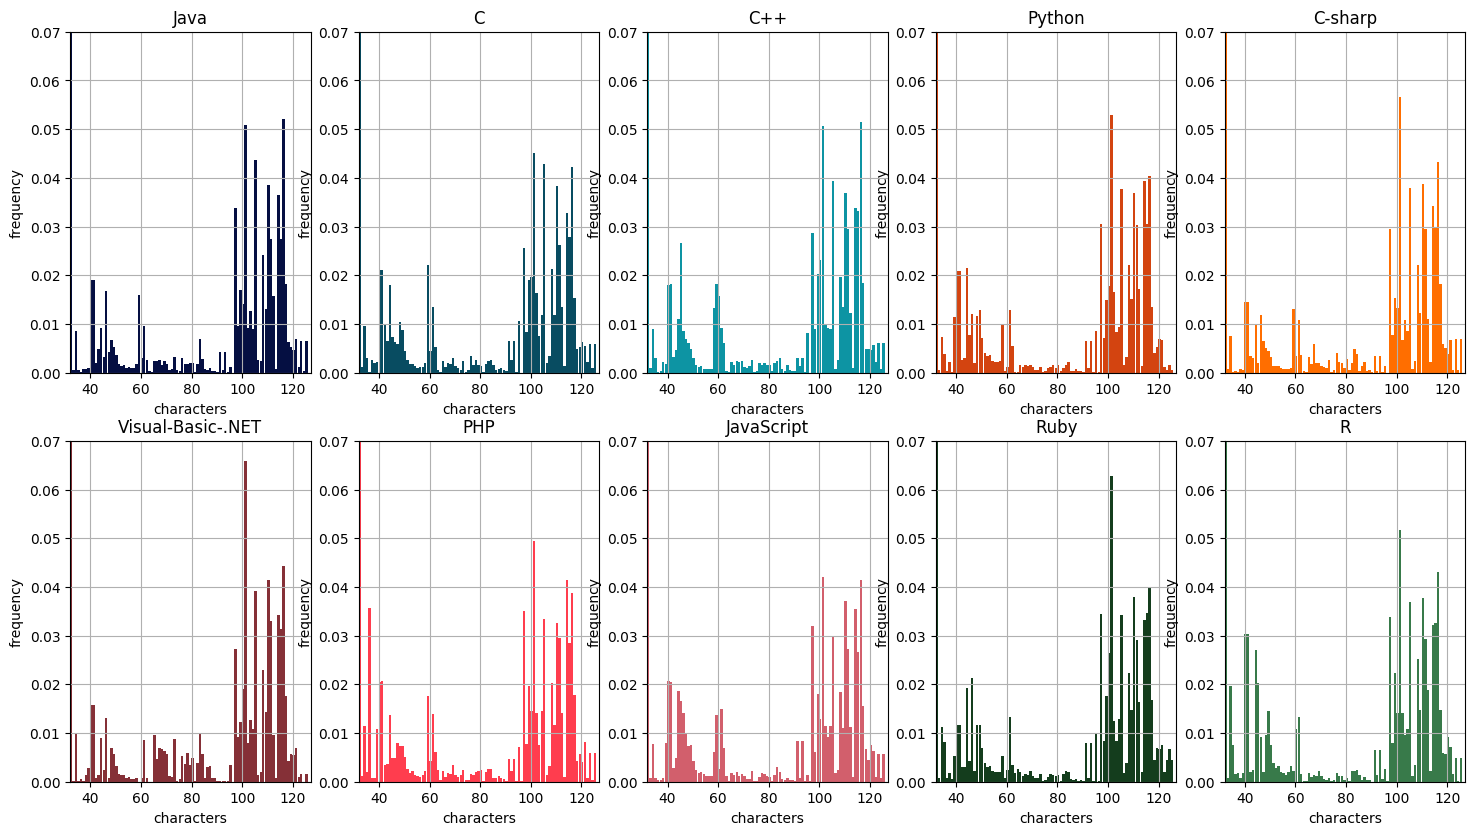
\includegraphics[width=6in]{frequencies}}
\end{center}
The character distributions of these languages are visually similar in terms of general shape. Each has relatively consistent letter frequencies, with letters like e, a, and s occurring more often than other letters, alphabetical characters appearing far more frequently than most punctuation, and spaces universally appearing most frequently of any character. However, looking closely at the data shows some trends upon which our network will ideally learn to base its decisions. Ruby, for example, uses comparatively few parentheses, which is reasonable given that its syntax uses those characters sparingly\footnote{Ruby, among other causes, does not require use of parentheses to call functions. Where most languages follow the convention of \mintinline{python}{function(x)}, Ruby permits use of \mintinline{ruby}{function x} notation.} compared to other languages. Additionally, curled braces (\texttt{\{\}}) dominate languages which use them to delineate code blocks. Python uses almost no semicolons, while those are common in most other languages, where they are used as statement terminators. Barely-noticeable differences abound, and what is difficult to see for a human can become quite obvious for a neural network.

Each character in this relevant range is counted within each training example of $1000$ characters. Input neurons receive a number in the range $[0,1]$ and use this data in forward propagation.

To build our network, we chain together four layers. The first (input) layer, will contain 94 total neurons: one for the frequency of each character we monitor.

The network contains two hidden layers of size 48 and 24 neurons. These sizes are relatively arbitrary; training would likely still succeed with other hidden layer sizes.

The output layer will contain 10 output neurons, expressing a probability $[0,1]$ that the code is written in each of the 10 languages.

\subsection{Results}
Though our network's predictions are not flawless, the network structure we propose is able to make predictions with an accuracy between 80 and 90\% depending on the layout of the data provided. To be specific, the network attained an accuracy of 84\% after taking roughly 16 seconds to train.

We can visualize the evolution of our network throughout the training process by looking to its accuracy and loss (cost function output) during the training process:

\begin{center}
    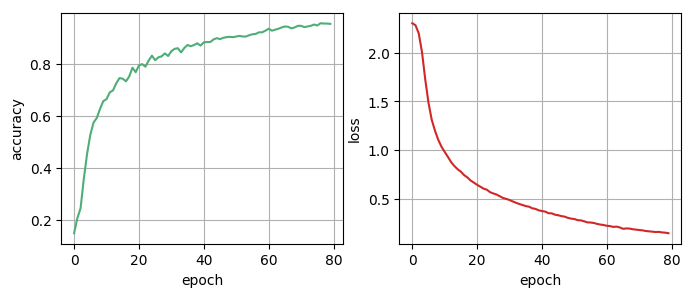
\includegraphics[width=5in]{history}
\end{center}

As one would expect, during training the network gradually improves as it learns through backpropagation how to perform language recognition. Similarly, the loss function decreases as the network starts to require less adjustment: when accuracy improves, the network will need less adjustment, and the cost function will decrease. Random guessing would yield an accuracy around 10\%, so the 85\% success rate our network was able to attain is relatively impressive.

\subsection{Future questions and improvements}
The network certainly is far from perfect, and future research is needed to refine the techniques expressed above. Concretely, a few opportunities for improvement are evident:
\begin{itemize}
    \item{In order to simplify the process of reading data, we concatenate all training samples for each language into one file, which is read in blocks of fixed length. This prevents the network from taking advantage of clear language indicators which would typically reside only at the start of a file. When lines between different files are blurred, we lose the ability to perform preliminary checks of language such as reading the interpreter path at the starting of an interpreted script. Future revisions could take into account the fact that code typically does not come in the form of 1000-character blocks.}
  \item{In order to increase the accuracy of this network implementation as well as its speed, a user may wish to implement a hybrid identification system involving attempts to determine language identity from file extensions, notable keywords, etc., then using the neural network if the less resource-intensive identification strategies fail.}
\end{itemize}

\section{Conclusion}
The success achieved through implementation of a deep neural network for classification of programming language demonstrates the ability of neural networks to accomplish the task of language classification. Our research builds upon preexisting research into natural language identification, applying modified techniques from that field. We show that neural networks can indeed extrapolate from minor and seemingly insignificant shifts in character frequency to make determinations on language identity in a manner similar to a human. Though there is room for improvement to the implementation discussed here and the techniques employed in this paper are nowhere near cutting-edge, this elementary research further shows that neural networks can emulate functions of human thought long thought irreproducible.

\section{Appendices}

\label{sec:appendix_a}
\subsection{Appendix A: Scripts for building training data}
Training and testing data for our neural network is retrieved from \url{http://rosettacode.org/}, a website which aggregates solutions to a wide variety of programming problems. This makes it an ideal source of diverse code using varied syntax.

Data is retrieved from an index on the code-sharing website GitHub\cite{rosettacodegh} using the script \texttt{download.sh}:
\inputminted{bash}{code/data/download.sh}

We used a simple Python script, \texttt{data\_reader.py}, to read raw text input and output a CSV file of training data for easy reading:
\inputminted{cpp}{"code/data_reader.py"}

\label{sec:appendix_b}
\subsection{Appendix B: Network Code}
All code for reading training data and performing training, backpropagation, and testing can be found in a file \texttt{network.py}.
\inputminted{python}{code/network.py}

All experimentation code was run on a desktop PC with 8GB RAM, an Intel Core i5-4460 3.20GHz CPU, and Arch Linux x86\_64.

\label{sec:appendix_c}
\subsection{Appendix C: Graphing Code}
Character frequency analysis graphs were generated with the following code:
\inputminted{python}{"code/data_graphs.py"}
Graphs of network performance were generated with this code:
\inputminted{python}{code/graphs.py}


\section{Acknowledgements}
I would like to thank Mr. William Snyder for serving as the adviser for this Extended Essay. Ms. Jamie Sample was the Extended Essay Coordinator for the GMHS IB students within the Class of 2019, and I'd like to thank her for tolerating my desire to use the most academic formatting possible in my essay. I'd also like to extend my regards to James Weichert for fighting through his \LaTeX-typeset essay on a similar topic alongside me, and for pointing me toward numerous terrific resources for grasping the mathematical technique behind neural networks. Finally, I'd like to give my most heartfelt gratitude to StackOverflow.com, without which I would never have reached the point of attempting a Computer Science EE in the first place.

\bibliography{research}

\end{document}
